\begin{figure*} 
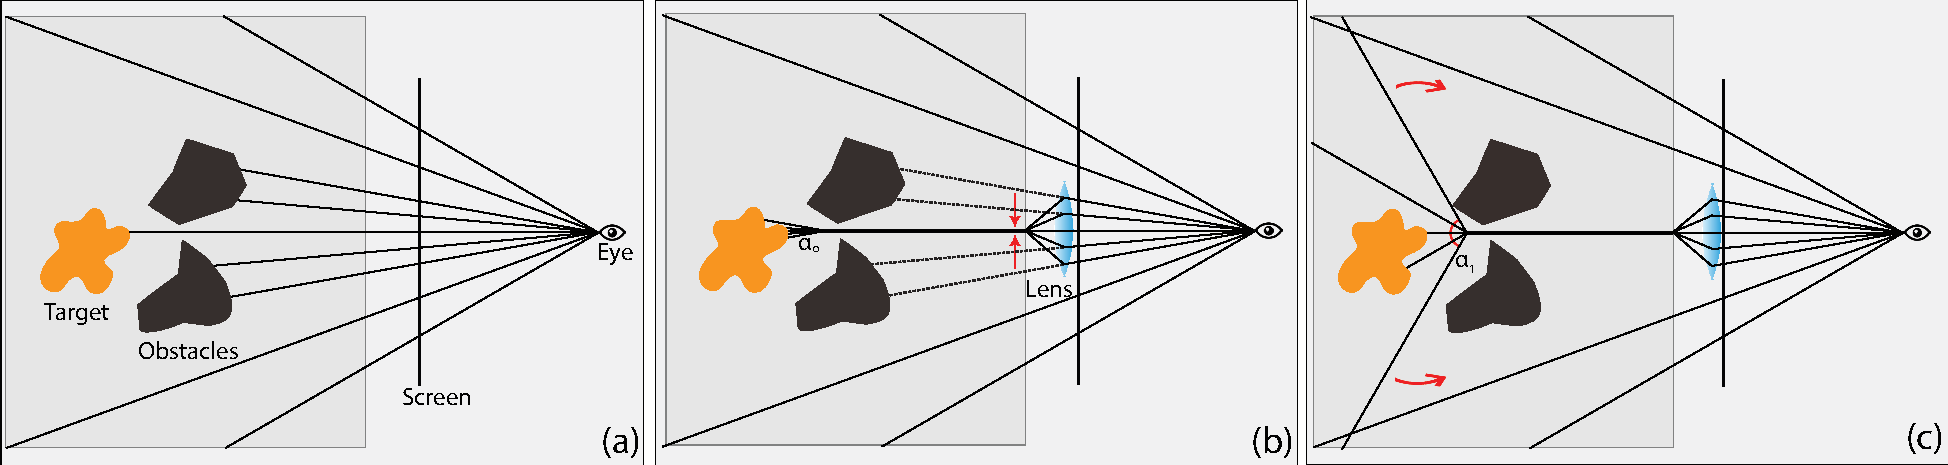
\includegraphics [width=\textwidth]{images/principle.pdf} 
\caption{The mechanism of the obstruction-free fish-eye lens. (a) The classic ray-casting where an interesting feature is partially hidden by other items in front of it. (b) The first main step: The lens makes converge the rays to avoid the obstacles. Once they are close to the target, the rays follow again their initial trajectory (with the initial angle) of view $\alpha_0$. Only a small part of the target is visible and magnified. (c) The target become visible by increasing the angle of view to $\alpha_1 \in \left[120,180\right]$.   }
\label{f:fisheye}
\end{figure*}


Direct volume rendering (DVR) is a pervasive visualization technique for displaying 3D scalar fields in many application fields such as engineering, material sciences, and medical imaging sciences. Recent DVR methods are able to display large such scalar fields at interactive rates and allow exploration of structures of interest. However widely adopted, and able to accommodate large volumes of data, DVR inherently suffers from the problem of \emph{occlusion}: Structures of interest located deep in the volume can be hard to spot and/or explore.

To aid with this, various mechanisms have been designed including transfer functions, segmentation, selection, and clipping. However, all such mechanisms have limitations.  \emph{Global} mechanisms, such as transfer function editing, can remove both occluders and objects of interest when these have similar densities. Moreover, in certain applications, carefully designed transfer functions exist and should be used without (significant) modifications to facilitate understanding and user training\,\cite{xxx}. \emph{Local} mechanisms such as segmentation, selection, or clipping are more effective in manipulating data confined to a given spatial region. However, many such mechanisms assume that one can easily and accurately select objects of interest to remove them (occluders) or keep them (occluded). This is hard to do when \emph{e.g.} one does not have direct access to the occluded objects, or when significant 3D interaction is required to select the occluder(s).

A different approach to handling occlusion is to use \emph{lenses}. Generically, these are flexible lightweight tools which enable local and temporary modifications of the DVR so as to reveal occluded objects while keeping the global visualization context~\cite{595268,CGF:CGF12871,xxx}. However, efficiently selecting the occluded object of interest and removing all in-between occluders in such contexts is still challenging \textbf{ALEX: Must explain FAR more clearly which are the limitations we address with our lens!}. 

In this paper, we propose to increase the flexibility of lenses for DVR exploration in several directions. We propose a focus-and-context (F+C) lens that combines a distortion technique, which pushes aside the occluding objects, with a fish-eye field of view in order to provide a better perspective on partially occluded items of interest in the volumes. We specifically target the use-case of \emph{partially occluded} objects, where the user has a glimpse of an interesting structure, buried deep within the data, and only slightly visible from a given viewpoint and transfer-function setting. We allow the user to `open up' the volume without changing these settings, and reveal the structure of interest, by a simple point, click, and scroll operation. Next, we provide several F+C modifications of the lighting parameters, transfer function, and geometry within the focus area so as to better understand the structure of interest. Our technique, implemented using a CUDA-based approach, can be easily incorporated in any generic DVR system.
 

%ALEX: Removed below text, it's not really related to our contribution here
%Furthermore, performances are still a  challenge in volume rendering systems. In fact, depending on the size of the dataset and also the resolution of the resulting produced image: the rendering process can be very slow. Some optimization strategies such as empty space skipping~\cite{Liu:2009:AVR:2421899.2421919}, early ray termination~\cite{CGF:CGF12605}, multiple and adaptive resolutions allow to speed up the rendering process by increasing the frame rate. With the advent of CUDA as a higher-level GPU programming language, CUDA-based ray-casters were introduced~\cite{Kainz:2009:RCM:1661412.1618498}. 


The structure of this paper is as follows. Section~\ref{sec:related_work} presents related work in occlusion management, lenses, and deformations for DVR visualization. Section~\ref{sec:principle} introduces our of our lens. Section 4 presents a method to convert vector datasets into a volume. Section 5 illustrates our lens technique with 3 scenarios. Section 6 discusses the presented technique. Finally, section 7 concludes the paper. 
